\section{Umsetzung}
\subsection{Technologie und Plattform}
In der Problembeschreibung zu dieser Arbeit wurden die Anforderungen an eine SmartHome Lösung diskutiert. In der anschliessenden Marktanalyse wurde openHAB als Grundlage zur Umsetzung unseres Projekts evaluiert. OpenHAB erfüllt die geforderten Kritierien, wie Herstellerunabhängigkeit, Installierbarkeit und Flexibilität. 
Für unser Projekt werden verschiedene Technologien bzw. Platformen eingesetzt. Auf der Clientseite, im SmartHome, wird openHAB mit verschiedenen Bindings eingesetzt. Cloudseitig wird MS Azure Cloud zur Persistierung von Events verwendet.

\subsection{openHAB}
Das System openHAB wird eingesetzt, um verschiedene Home-Automatisierungssysteme unter einen Hut zu bringen. Um dies zu realisieren bietet openHAB eine grosse Anzahl von Bindings mit, mit denen die verschiedenen Systeme angesprochen werden können.

\subsubsection{Module}
OpenHAB ist durch OSGi-Bundles modular aufgebaut und binhaltet folgende Komponenten:

\begin{figure}[H]
	\centering
		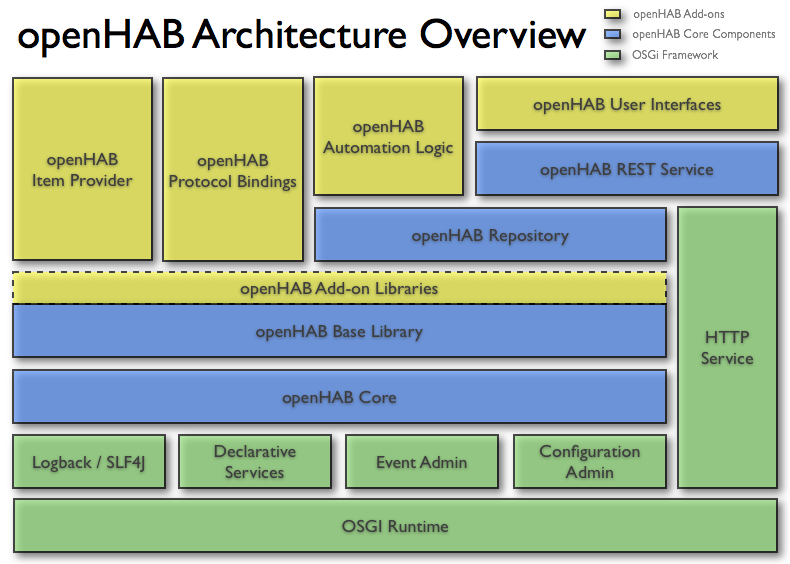
\includegraphics[scale=0.45]{report/img/openHAB_architecture}
	\caption{openHAB Architektur}
	\label{fig:ohArch}
\end{figure}


\subsubsection{Kommunikation}
Der Basisservice von openHAB stellt der Event Bus dar. Über diesen Bus werden Events zwischen den verschiedenen Bundles gesendet. Die Events sind entweder Commands, welche eine Aktion ausführen, oder Status-Updates, welche Statusänderungen der Devices beinhaltet. \\
Durch den Einsatz dieses EventBus wird die Kopplung reduziert und können somit einfach ausgetauscht werden. \\
Für die Verwaltung der verschiedenen Status ist das Item Repository zuständig, welches permanent den Event Bus auf Status-Updates abhört und die Änderungen ins Repository schreibt. Falls auf einem GUI ein Status eines Devices angezeigt werden soll, kann dazu das Item Repository abgefragt werden.\\
Das Repository persistiert die Status und ist somit auch nach einem Neustart verfügbar.

\begin{figure}[H]
	\centering
		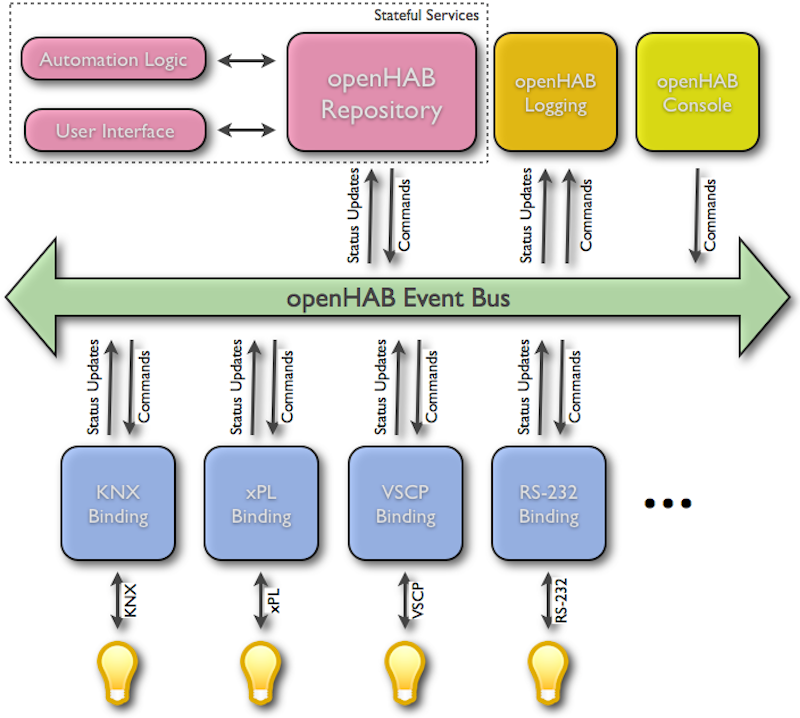
\includegraphics[scale=0.4]{report/img/communicationOH}
	\caption{Kommunikation openHAB}
	\label{fig:ohComm}
\end{figure}

\subsubsection{Bindings}
Ein Binding ist eine Verbindung zwischen dem Event Bus und den externen Systemen. Diese Verbindungen sind aufgrund der verschiedenen Technologien verschieden. Dadurch muss für jede Technologie ein eigenes Binding geschrieben werden. Für einige Systeme sind Bindings vorhanden, die einzeln heruntergeladen und als «Add-on» installiert werden können.
Die Bindings stellen nur sicher, dass Events zwischen Event Bus und den jeweiligen Devices ausgetauscht werden können. Sie müssen sich also nicht um Statusänderungen oder ähnliches kümmern, da dies durch das Item Repository übernommen wird. \\
Alle momentan verfügbare Bindings sind unter folgendem Link zu finden: \url{https://github.com/openhab/openhab/wiki/Bindings}

\pagebreak

\subsection{Installation openHAB}



\subsection{Deploymentübersicht}

\subsubsection{Binding Azure}
\begin{figure}[h!]
	\centering
		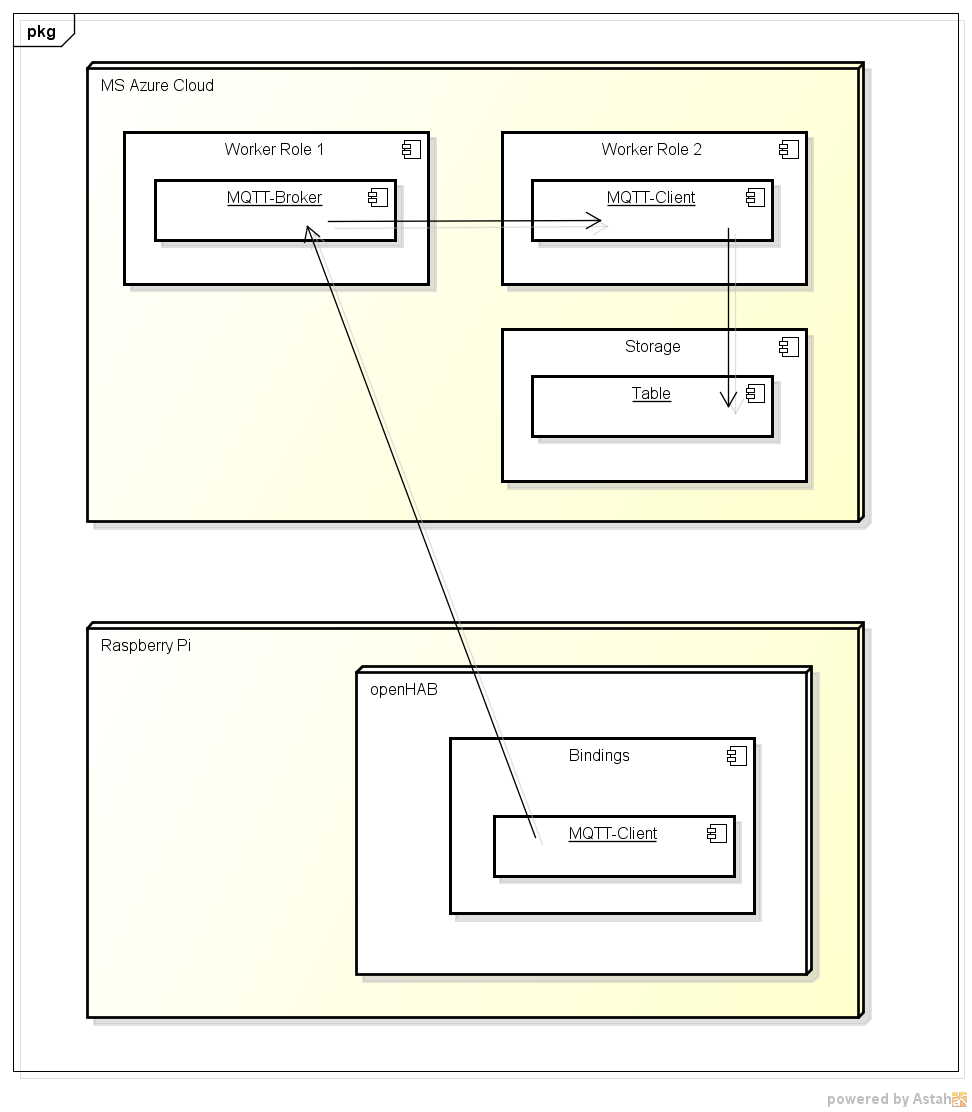
\includegraphics[scale=0.5]{report/img/deployment_binding_azure}
	\caption{Binding Azure Cloud}
	\label{fig:deploymentAzure}
\end{figure}

\subsubsection{MQTT Binding}

\subsection{MQTT}
MQTT steht für «Message Queue Telemetry Transport» und ist ein Nachrichten-Protokoll, das speziell für IOT-Anwendungen konzipiert wurde. Es setzt auf dem TCP/IP Stack auf und wird für den Nachrichtenaustausch zwischen verschiedenen, verteilten Maschinen verwendet. \\
Das Protokoll wurde speziell für Systeme designt, die über wenig Speicherplatz und kleiner Netzwerk-Bandbreite verfügen, was bei IOT-Anwendungen meist der Fall ist.

\subsubsection{Funktionsweise}
MQTT folgt dem Prinzip «Publish/Subscribe», sprich Clients können bestimmte Topics abonnieren. Wenn Messages auf dieses Topic gesendet werden, leitet der Broker diese an alle interessierten Clients weiter. \\
In Bezug auf erstellen von Topics agiert der Broker passiv. Das bedeutet, Clients können sich auf beliebigen, selber defnierte, Topics registrieren. Wenn aber niemand auf dieses Topic publiziert, wird der Client nie eine Message erhalten.

\begin{figure}[h!]
	\centering
		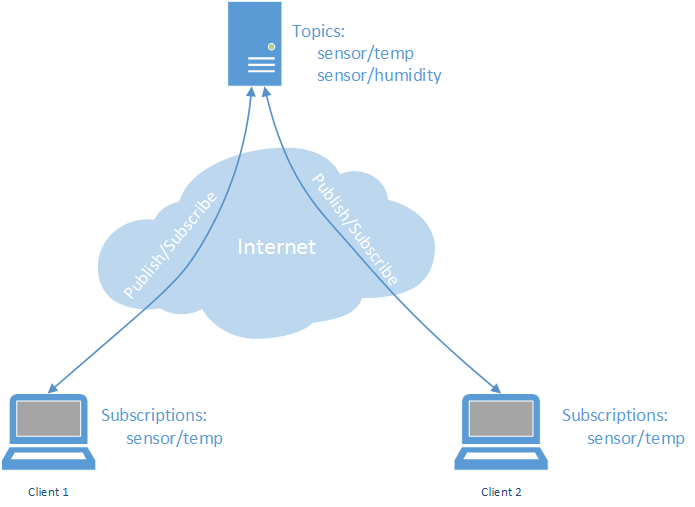
\includegraphics[scale=0.6]{report/img/mqttFunktionsweise}
	\caption{Funktionsweise MQTT}
	\label{fig:deploymentAzure}
\end{figure}






